\documentclass[10pt,a4paper]{article}

\usepackage[utf8]{inputenc}

\usepackage{amsmath}

\usepackage{amsfonts}

\usepackage{amssymb}

\usepackage{graphicx}

\usepackage{natbib}

\newcommand{\x}{\mathbf{x}}

\newcommand{\y}{\mathbf{x}_o}

\newcommand{\z}{\mathbf{x}_z}

\newcommand{\vomega}{\vec{\omega}}

\title{On BSSRDF estimation}

\date{January 2018}

\author{Alessandro Dal Corso \\ Technical University of Denmark \and Jeppe Revall Frisvad \\ Technical University of Denmark}



\begin{document}

\maketitle



\begin{figure}[h]

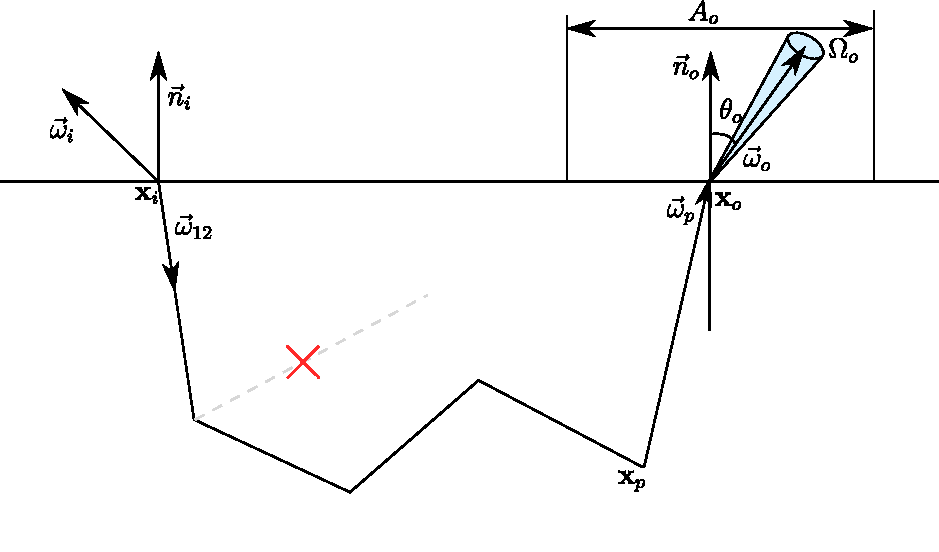
\includegraphics[scale=0.7]{configuration_pt.pdf}
\vspace{-5ex}
\caption{Configuration for random walk procedure.}

\label{fig:diagram_pt}

\end{figure}

\noindent The configuration of the bidirectional scattering-surface reflectance distribution function (BSSRDF) is illustrated in Figure~\ref{fig:diagram_pt}. Our aim is to estimate the BSSRDF for a specific spatial area bin with area $A_o$ and for a specific angular bin with solid angle $\Omega_o$. In a measurement environment~\cite{venable74}, we have the following incident flux:
%
\[
\Phi_i(A_i, \Omega_i) = \int_{A_i} \int_{\Omega_i} L_i(\x_i', \vomega_i') (\vomega_i' \cdot \vec{n}_i) \, d\omega_i' \, dA_i' \, ,
\]
%
where $L_i$ is radiance incident somewhere on the surface area $A_i$ from the solid angle $\Omega_i$. As illustrated in Figure~\ref{fig:diagram_pt}, $\vec{n}_i$ is the surface normal at a point of incidence $\x_i'$, while $\vomega_i'$ is a direction of incidence. The corresponding responsivity-weighted emergent flux is:
%
\[
\Phi_o(A_o, \Omega_o) = \int_{A_o} \int_{\Omega_o} \int_{A_i} \int_{\Omega_i} L_i(\x_i', \vomega_i') S(\x_i', \vomega_i', \x_o', \vomega_o') R(\x_o', \vomega_o') (\vomega_i' \cdot \vec{n}_i) \, d\omega_i' \, dA_i \, (\vomega_o' \cdot \vec{n}_o) \, d\omega_o' \, dA_o' \, ,
\]
%
where $R$ is the relative responsivity of the instrument used for a measurement and $S$ is the BSSRDF. Note that we choose our notation so that $\Phi_o(A_o, \Omega_o)$ represents the emergent flux arriving in the bin of interest. In an idealized computational setting, we ignore the responsivity of the sensor and set $R(\x_o', \vomega_o') = 1$. If we choose a unit response function and unit incident radiance $L_i(\x_i, \vomega_i) = \delta(\x_i - \x_i')\delta(\vomega_i - \vomega_i')$, the ratio of emergent to incident flux is
%
\[
\rho(A_o, \Omega_o) = \frac{\Phi_o(A_o, \Omega_o)}{\Phi_i(A_i, \Omega_i)} =  \int_{A_o} \int_{\Omega_o} S(\x_i, \vomega_i, \x_o', \vomega_o') (\vomega_o '\cdot \vec{n}_o) \, d\omega_o' \, dA_o' \, .
\]

Once we have obtained $\rho$, we can rearrange the above equation to obtain the BSSRDF of a bin with $\x_o \in A_o$ and $\vomega_o \in \Omega_o$:
%
\begin{equation}
S(\x_i, \vomega_i, \x_o, \vomega_o) = \frac{d L_o(\x_o, \vomega_o)}{d\Phi_i(\x_i, \vomega_i)} \approx \frac{\Phi_o(A_o, \Omega_o)}{\Phi_i(A_i, \Omega_i) A_o \Omega_o (\vec{\Omega}_o \cdot \vec{n}_o)} = \frac{\rho(A_o, \Omega_o)}{ A_o \Omega_o (\vec{\Omega}_o \cdot \vec{n}_o)} \ ,
\label{eq:bssrdf}
\end{equation}
%
where $\vec{\Omega}_o$ is the direction around which the bin solid angle is centered. This means that we can represent the light scattering between two points, that is, the BSSRDF, as the ratio of emergent to incoming flux divided by the projected area and the solid angle.

The BSSRDF of a medium can be defined as an operator that includes all radiance resulting from the scattering events in the medium~\citep{preisendorfer65}. This radiance is described locally by the radiative transfer equation~\citep{preisendorfer65}. Thus, we can evaluate the scattering process given by the BSSRDF using the radiative transfer equation. So, the reflectance quantity $\rho$ becomes the ratio of flux carried by a flux packet that arrives in a bin after going through a random walk. This is the procedure used by Wang et al.~\cite{wang1995}.

The random walk procedure works as follows:
%
\begin{enumerate}

\item Create a new photon with flux $\Phi_t = 1 / N$, where $N$ is the number of photons. Start assigning $\x_p = \x_i$ and $\vomega_p = \vomega_{12}$, the refracted incoming direction.

\item Sample a new distance to the next scattering event $s$. We assume a homogenous medium, so we use an exponential distribution with decay $\sigma_t$, that can be easily importance sampled:
%
\[
s = \frac{-\log(1 -\xi)}{\sigma_t} \, , \quad \textrm{with $\xi \in [0,1)$.}
\]

\item Check if the next scattering event $\x_p' = \x_p + s \vomega_p $ is within the medium.

\item If the next scattering event is within the medium:

\begin{enumerate}

\item Terminate the path with probability $1-\alpha$. If terminated, start from step~1.

\item If not terminated, sample a new direction $\vomega_p$ according to the phase function.

\item Continue from step 2.

\end{enumerate}

\item If the next scattering event is outside of the medium:

\item Calculate the reflection Fresnel coefficient $R_{21}$ and update $\x_p$ to be the intersection point on the surface of the medium.

\begin{enumerate}

\item With probability $R_{21}$ reflect the path around $-\vec{n}_o$, and continue from step~2.

\item With probability $1 - R_{21}$ refract the path outside, storing $\Phi_t$ in the corresponding bin. Start from step 1.

\end{enumerate}

\end{enumerate}

Note that all the sampling is chosen to cancel out the terms that would change the stored flux. So, the flux within the medium should change for each scattering event as:
%
\[
\Phi_t' = \Phi_t \sigma_s p(\vomega_p \cdot \vomega_p) e^{-\sigma_t s} \, .
\]
%
Although, dividing by the pdfs, $p(\vomega_p \cdot \vomega_p')$ cancels out if we sample $\vomega_p$ according to the correct phase function, $e^{-\sigma_t s}$ cancels with the pdf of the distance sampling, leaving $\sigma_s/\sigma_t = \alpha$. This last factor is divided out by the path continuation probability, leading to $\Phi_t' = \Phi_t$ as expected. If the flux goes outside the medium, the Fresnel coefficients cancel with the probabilities of reflection or transmission.



\section{Variance reduction through connections}

\begin{figure}[h]

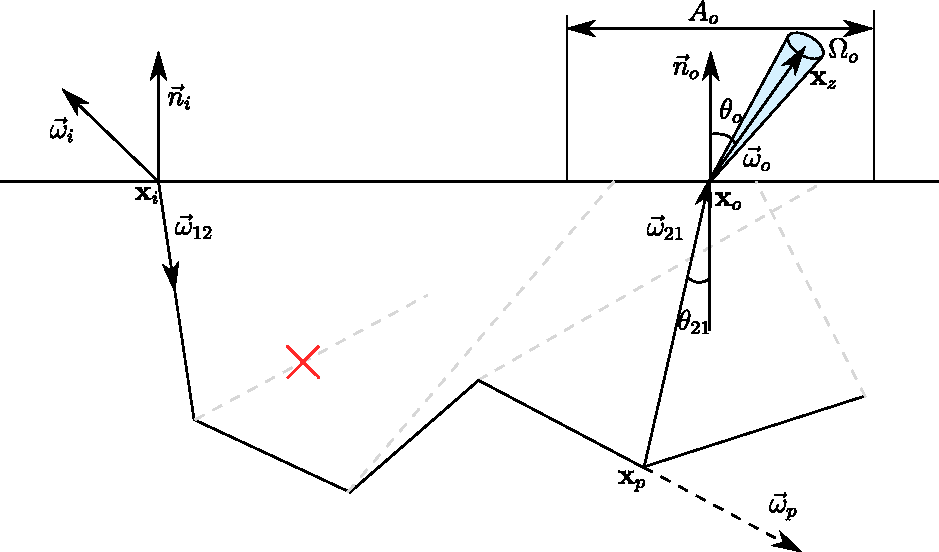
\includegraphics[scale=0.7]{configuration.pdf}\\[-4ex]

\caption{Configuration for the connection event described in the text.}
\label{fig:diagram}

\end{figure}



\noindent The procedure from the previous section provides an unbiased estimate of the BSSRDF. However, this process requires a huge number of photons to converge to an acceptable solution. To reduce convergence times, we connect each scattering event (except the first, if we measure multiple scattering only), to a point $\x_o$ on the surface. We then use the three point form of the local scattering equation~\cite{raab08} to calculate the resulting measurement:
%
\[
L(\x_o, \vomega_o) =  L_e(\x_o, \vomega_o) + L(\x_p \rightarrow \x_o) f(\x_p \rightarrow \x_o \rightarrow \x_z) G(\x_p \leftrightarrow \x_o) V(\x_p \leftrightarrow \x_o) \, .
\]

We assume a non emissive body ($L_e(\x_o, \vomega_o) = 0$). In our case, we have a point in the volume generating a scattering event ($\x_p$), a point in a bin on the surface ($\y$), and a point specifying a direction into the bin ($\z$), see Figure~\ref{fig:diagram}. So, we have the incoming radiance:
%
\[
L(\x_p \rightarrow \y) = \alpha \Phi_t(\mathbf{x}_p) p(\vomega_p \cdot \vomega_{21}, g) \, ,
\]
%
the three point scattering function corresponding to the bidirectional transmittance distribution function (BTDF) of a perfectly smooth surface~\cite{pharr17}:
%
\begin{eqnarray}
f(\x_p \rightarrow \y \rightarrow \z) & = & T_{21}(\eta, \vomega_o) \frac{\delta(\vomega_o - \vomega_t)}{|\vomega_{21}\cdot\vec{n}_o|} \, , \label{eq:btdf} \\
\vomega_t & = & \eta^{-1}(\vomega_{21} - (\vomega_{21}\cdot\vec{n}_o)\vec{n}_o) + \vec{n}_o \sqrt{1 - \eta^{-2}(1 - (\vomega_{21}\cdot\vec{n}_o)^2)} \, , \nonumber
\end{eqnarray}
%
the geometry term:
%
\[
G(\x_p \leftrightarrow \y) = \frac{|\vomega_{21}\cdot\vec{n}_o |}{\|\y - \x_p\|^2} \, ,
\]
%
and the generic visibility term:
%
\[
V(\x_p \leftrightarrow \y) = V'(\x_p \leftrightarrow \y) \exp\left(-\int_0^{\|\y - \x\|} \sigma_t\left(\x_p + t \vomega_{21}\right) dt\right) .
\]
%
Here, $T_{21} = 1 - R_{21}$ is the Fresnel transmittance at the point of emergence, and one should note that $T_{21}(\eta^{-1}, -\vomega_{21}) = T_{21}(\eta, \vomega_o)$. In addition, we disregard (de)compression of solid angle in the BTDF, as we consider light incident and emergent in the same medium only, so the compression cancels out upon emergence.

In our configuration of a semi infinite plane, the binary visibility function $V'(\x_p \leftrightarrow \y)$ is always one (i.e., it is always possible to connect to the emergent point). Since we have a homogenous medium, we can rewrite $V$ as the beam transmittance:
%
\[
V(\x_p \leftrightarrow \y) = \exp(-\sigma_t \|\y - \x_p\|) \, .
\]
%
And the radiance of the $p$th scattering event of the $k$th photon becomes
%
\[
L_{k,p}(\x_o, \vomega_o) = \alpha \Phi_t(\mathbf{x}_p) p(\vomega_p \cdot \vomega_{21}, g)  T_{21}(\eta, \vomega_o) \frac{\delta(\vomega_o - \vomega_t)}{\|\y - \x_p\|^2} \exp(-\sigma_t \|\y - \x_p\|) \, .
\]

To get the collective contribution of a photon path, we need to sum all the elements of the random walk:
%
\[
L_k(\x_o, \vomega_o) = \sum_p L_{k,p}(\x_o, \vomega_o) \, .
\]
%
And to get the final emergent flux, we need to solve the measurement equation for each bin. This is integration of incident flux (given by the three point form of the local scattering equation) across the cosine-weighted area and the solid angle of the bin:
%
\[
\Phi_o(A_o, \Omega_o) = \int_{A_o} \int_{\Omega_o} L(\x_o', \vomega_o') (\vomega_o' \cdot \vec{n}_o) \, d\omega_o' \, dA_o' \, .
\]

Now, since the three point scattering function (\ref{eq:btdf}) is a delta function with respect to direction, the integration over bin solid angle cancels with this delta. As for the area integral, we solve it using Monte Carlo integration with $\x_o$ sampled in polar coordinates:
%
\[
\Phi_o(A_o, \Omega_o) = \frac{1}{M} \sum_{q = 1}^M \sum_{k = 1}^N \frac{L_k(\x_{o,q}, \vomega_t) w(\Omega_o, \vomega_t) \|\x_{o,q} - \x_i\|}{\text{pdf}(\x_{o,q})} \, ,
\]
% 
where $w(\Omega_o, \vomega_t)$ is 1 if $\vomega_t \in \Omega_o$ and 0 otherwise. Using just one area sample per bin per progressive update ($M = 1$, $\x_{o,q} = \x_{o,1} = \x_o'$) and recalling that $\Phi_t = 1/N$, the estimator becomes
%
\[
\Phi_o(A_o, \Omega_o) = \frac{\alpha}{N} \sum_{k=1}^N\sum_p p(\vomega_p \cdot \vomega_{21}, g) T_{21}(\eta, \vomega_t)  \frac{\vomega_t \cdot \vec{n}_o}{\|\x_o' - \x_p\|^2}  e^{-\sigma_t \|\x_o' - \x_p\|} \frac{\|\x_o' - \x_i\|}{\text{pdf}(\x_o')} w(\Omega_o, \vomega_t) \, ,
\]
%
where we sample $\x_o'$ uniformly in polar coordinates. If we think of our spatial bin $A_o$ as a circular sector delimited by $r_\text{min}$ and $r_\text{max}$ in radius, and $\theta_{s,\text{min}}$ and $\theta_{s,\text{max}}$. We have $\text{pdf}(\x_o') = 1/(\Delta r \Delta \theta_{s})$, where $\Delta r =  r_\text{max} - r_\text{min}$ and $\Delta \theta_{s} = \theta_{s,\text{max}} - \theta_{s,\text{min}}$.  Since we use a circular sector, we obtain:
%
\[
A_o = \int_{A_o} dA = \int_{r_\text{min}}^{r_\text{max}}\int_{\theta_{s,\text{min}}}^{\theta_{s,\text{max}}} r dr d\theta_s =  \frac{r_\text{max}^2 - r_\text{min}^2}{2}  \Delta \theta_{s} = \frac{r_\text{min} + r_\text{max}}{2}  \Delta r \Delta \theta_{s} \, .
\]
%
Also, since we are using a uniform sampling of the hemisphere, we obtain a constant solid angle for all directional bins:
%
\begin{equation*}
\Omega_o = \frac{2\pi} {N_{bins}} \, .
\end{equation*}

Plugging everything into the original BSSRDF equation~(\ref{eq:bssrdf}) and simplifying, we obtain the final BSSRDF estimate:
%
\begin{equation*}
\begin{split}
S(\x_i, \vomega_i, \x_o, \vomega_o) = &\frac{\alpha}{N} \sum_{k=1}^N\sum_p p(\vomega_p \cdot \vomega_{21}, g)  \frac{ T_{21}(\eta, \vomega_t)}{\vec{\Omega}_o \cdot \vec{n}_o}  \frac{\vomega_t\cdot\vec{n}_o}{\|\x_o' - \x_p\|^2}  e^{-\sigma_t \|\x_o' - \x_p\|} \\& {\|\x_o' - \x_i\|} \frac{2}{r_\text{min} + r_\text{max}} \frac{N_{bins}}{2\pi} w(\Omega_o, \vomega_t)
\end{split}
\end{equation*}
%
for $\x_o \in A_o$ and $\vomega_o \in \Omega_o$.
%Note that we used $\Phi(\x_i, \vomega_i) = 1$.



\bibliographystyle{plain}

\bibliography{bssrdf_note}



\end{document} 